\chapter{Materiais e métodos}\label{cap:metodos}

Em 2 de novembro de 2026, o sistema descrito na seção~\ref{cap:sistema} adquiriu \campoJanelasOperacao\ janelas de sinal bruto em \campoEnsaios\ ensaios de \campoMaquinas\ máquinas de uma instalação industrial, todas em operação normal, além de \campoJanelasMotorParado\ janelas com o motor desligado e \campoJanelasRepouso\ janelas com o transmissor parado sobre uma mesa. Com esses dados, a detecção de falhas por afastamento da operação normal foi avaliada por três hipóteses, cada uma com critérios de corroboração e de refutação (seção~\ref{sec:hipoteses}). A primeira trata do falso alarme entre duas rodadas da mesma máquina, a segunda, da menor mudança detectável na velocidade eficaz, e a terceira, da detecção de uma assinatura de desbalanceamento somada a janelas reais. Uma quarta hipótese avaliou o mesmo detector numa base pública de laboratório, com desbalanceamento real.

\section{Local, máquinas e ensaios}\label{sec:ensaios}

As quatro máquinas são uma dobradeira, uma guilhotina hidráulica, uma calandra piramidal e um compressor de parafuso (Figura~\ref{fig:maquinas}), no mesmo galpão (Figura~\ref{fig:planta}). A calandra está no nível 2 do galpão, e as outras três máquinas, no nível 1. O compressor fica numa sala própria, junto à parede externa. A empresa responsável pela instalação autorizou a coleta e a publicação das fotos. Segundo o operador, todas estavam saudáveis e operaram sem carga durante os ensaios. Nas duas placas de motor legíveis, a da guilhotina e a da calandra, os motores são de indução trifásicos de \SI{60}{\hertz}, com rotação nominal de \SI{1760}{r/min} e de \SI{1715}{r/min} (Tabela~\ref{tab:ensaios}). Na guilhotina, o motor gira continuamente, e um pedal aciona a lâmina; os acionamentos da lâmina durante os ensaios não foram anotados.

\begin{figure}[!htb]
\centering
\caption{Máquinas da coleta em campo}\label{fig:maquinas}
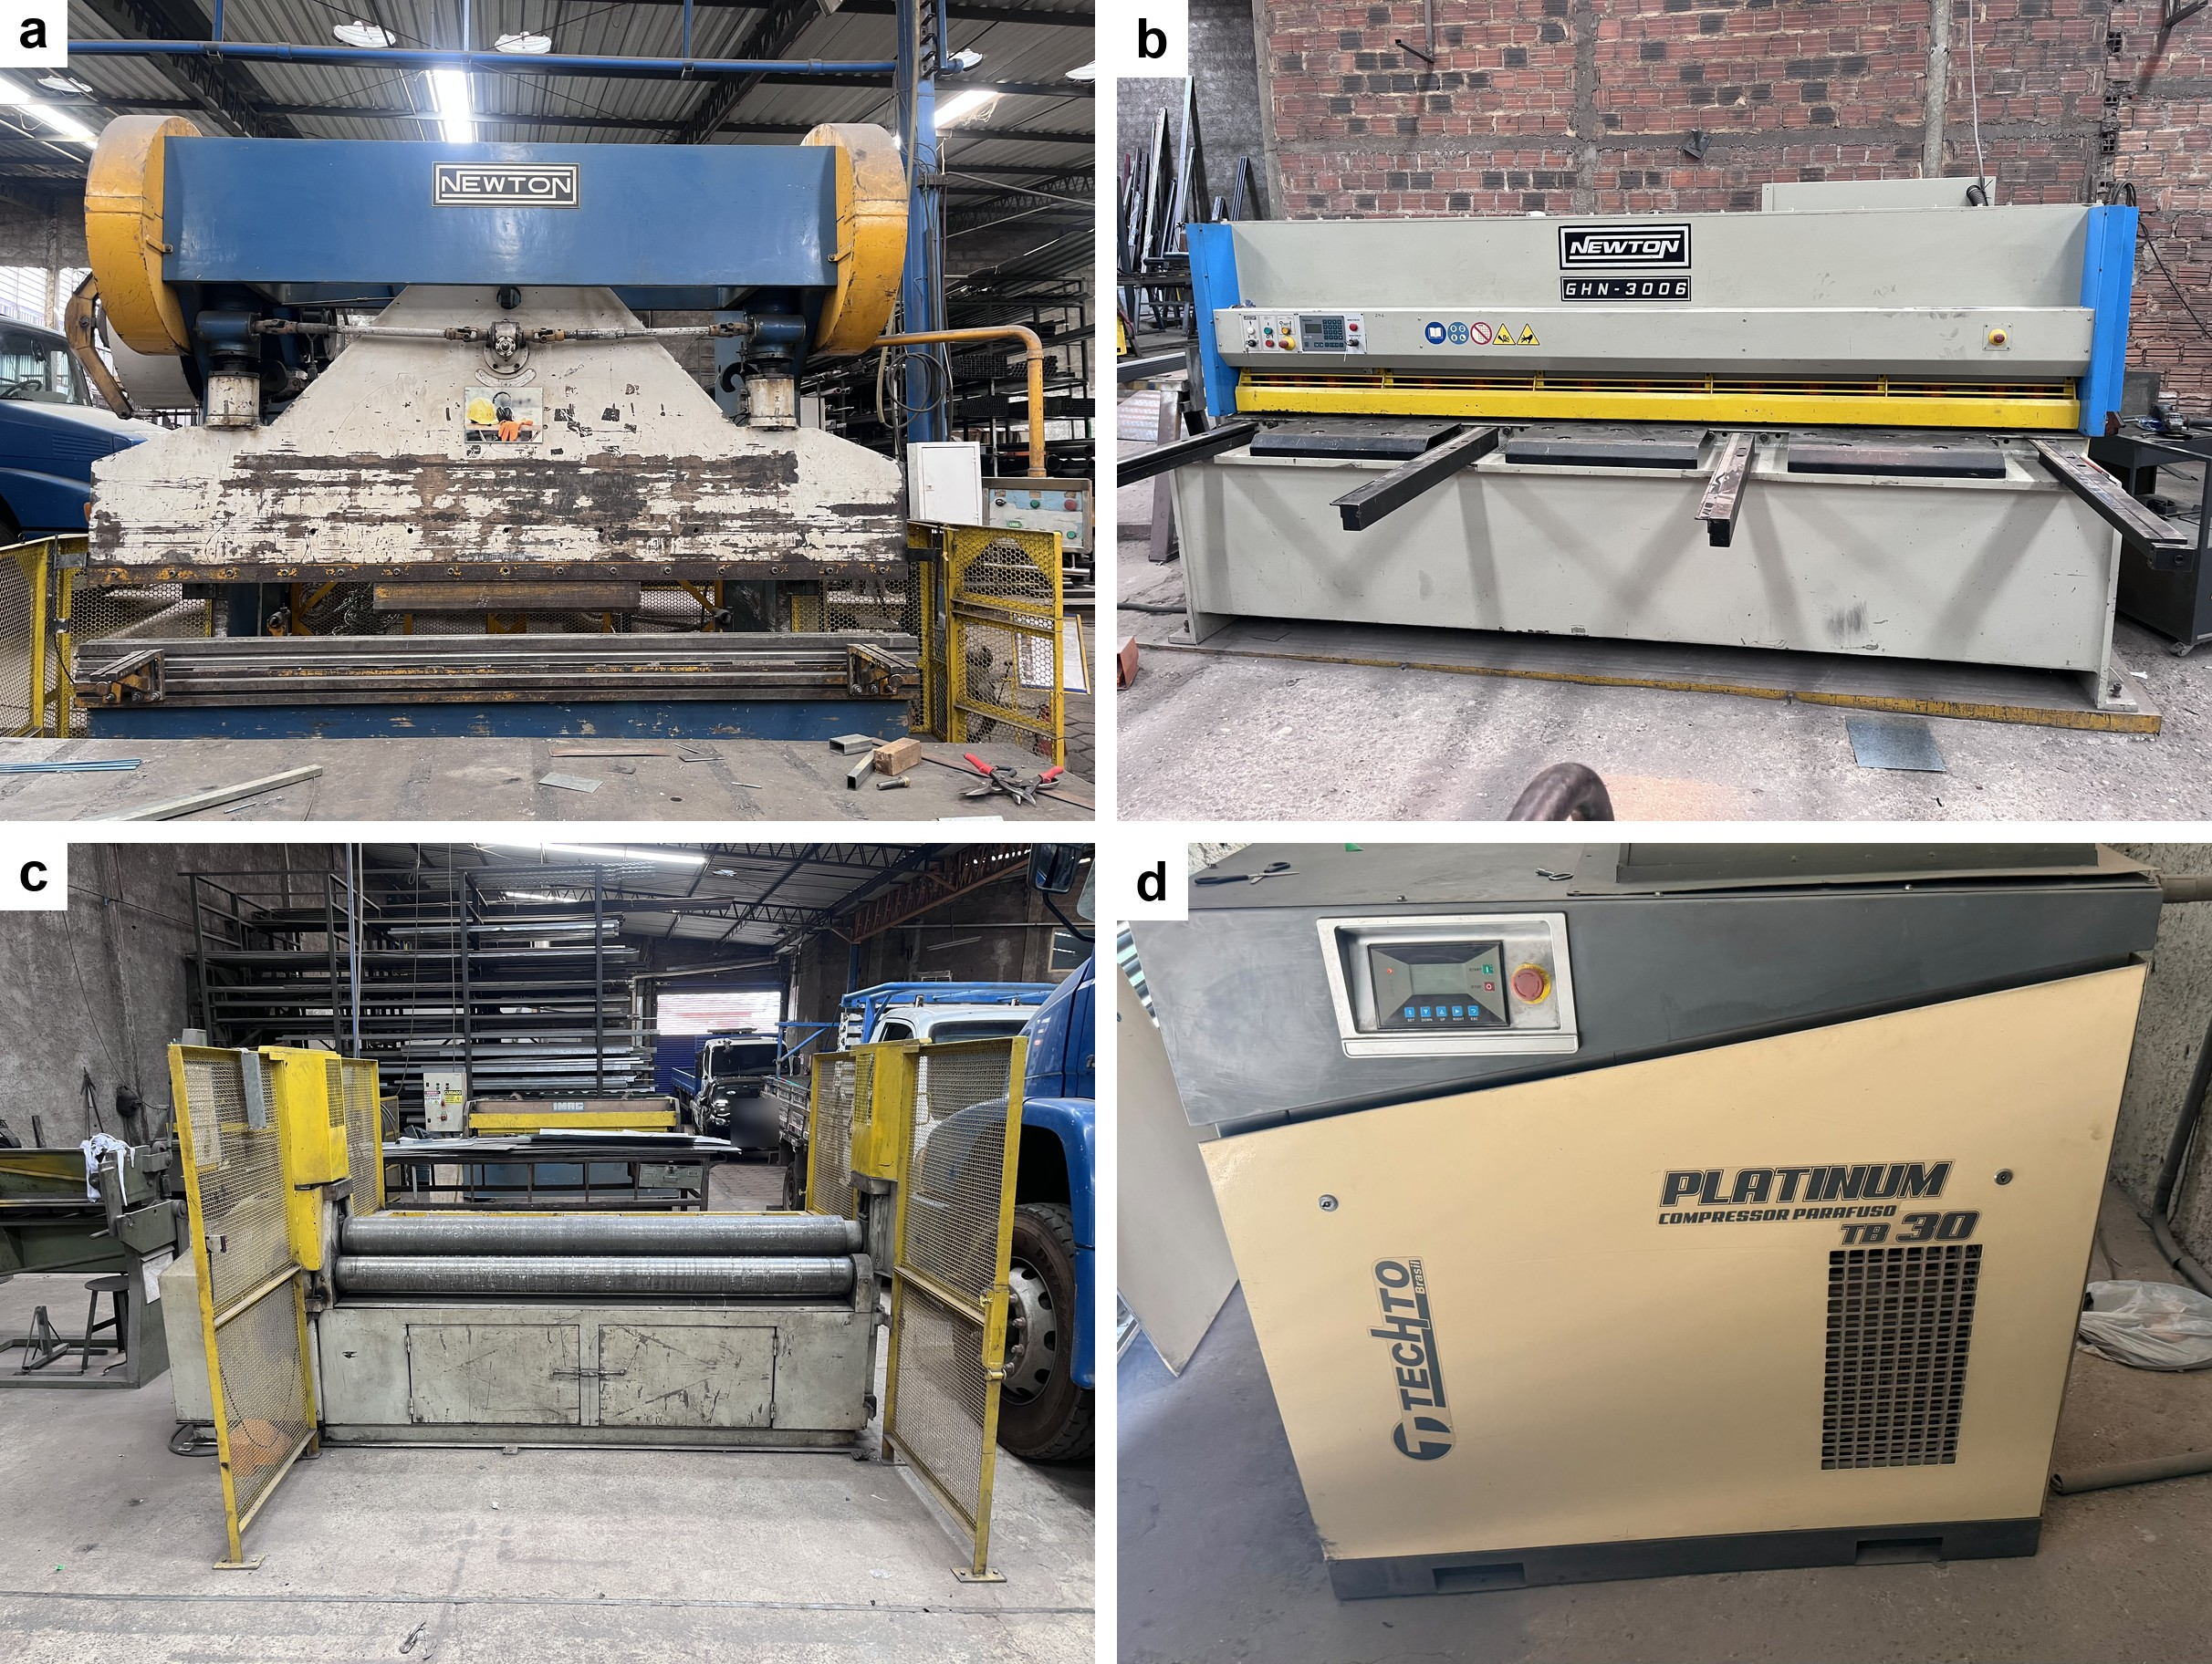
\includegraphics[width=\textwidth]{campo/fig19_maquinas.jpg}
\fonte{elaborado pelo próprio autor.}
\legenda{(a) dobradeira Newton PDM; (b) guilhotina hidráulica Newton GHN-3006; (c) calandra piramidal Vega CPVG2050X14; (d) compressor de parafuso Techto TB~30, fechado. Fotos de 2 de novembro de 2026. Em (c), a placa de um veículo e um logotipo, ao fundo, foram desfocados.}
\end{figure}

\begin{figure}[!htb]
\centering
\caption{Planta esquemática do galpão da coleta em campo}\label{fig:planta}
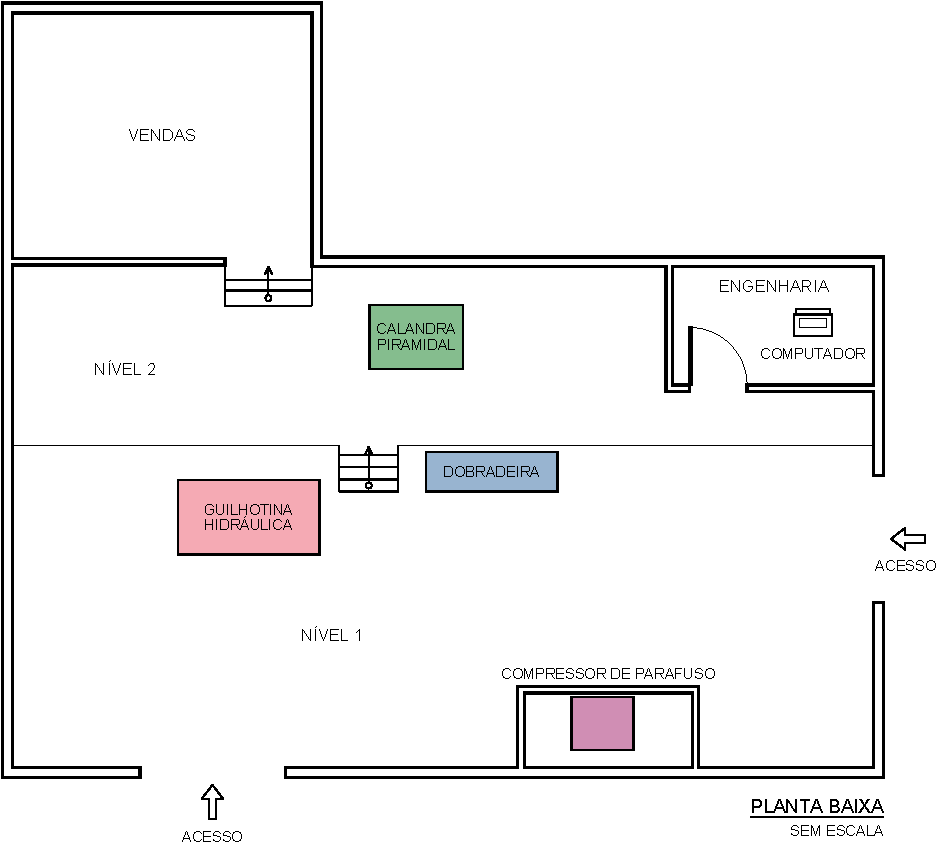
\includegraphics[width=\textwidth]{fig21_planta_local.pdf}
\fonte{elaborado pelo próprio autor.}
\legenda{planta sem escala, com as proporções de um esboço do autor. A linha fina entre os níveis 1 e 2 marca a mudança de nível do piso. Nas escadas, a linha começa num círculo e termina em seta no sentido da subida. As setas externas indicam as duas entradas do galpão. Cada máquina tem, em tom claro, a cor que a identifica nas Figuras~\ref{fig:ruido}, \ref{fig:espectros}, \ref{fig:injecao} e~\ref{fig:ap1}. O transmissor e o \textit{gateway} foram levados de uma máquina a outra e não têm posição fixa na planta.}
\end{figure}

A coleta teve duas rodadas. A primeira foi das \campoInicioDobradeiraUm\ às \campoFimCompressorUm, com um ciclo a cada \campoCicloUm~s, e a segunda, das \campoInicioCalandraDois\ às \campoFimGuilhotinaDois, com um ciclo a cada \campoCicloDois~s, depois de uma tentativa na dobradeira durante os reinícios do transmissor, das \reiniciosInicio\ às \reiniciosFim. Em cada ciclo, o transmissor enviou uma telemetria e uma janela de sinal bruto de \SI{0,512}{\second}, de modo que as janelas cobrem de \campoCoberturaUm~\% a \campoCoberturaDois~\% do tempo de cada ensaio. A calandra e a guilhotina foram medidas nas duas rodadas, com \campoIntervaloCalandra\ e \campoIntervaloGuilhotina\ entre os inícios dos dois ensaios de cada uma. Na segunda rodada, a dobradeira não teve sinal bruto, porque o transmissor, alimentado desde a manhã por uma bateria que não tinha sido carregada antes da coleta, reiniciou a cada ciclo por queda de tensão. Nos ensaios seguintes, ele foi alimentado por um carregador portátil. A temperatura do sensor, informada na telemetria, teve mediana de \campoTempRodadaUmMin~\si{\celsius} a \campoTempRodadaUmMax~\si{\celsius} nos ensaios da primeira rodada e de \campoTempRodadaDoisMin~\si{\celsius} a \campoTempRodadaDoisMax~\si{\celsius} nos da segunda, já com o carregador.

Os trechos analisados excluem a partida dos motores e o tempo em que a gravação continuou depois do fim da operação (Tabela~\ref{tab:ensaios}). Eles foram delimitados em 2 de novembro, nas análises exploratórias (seção~\ref{sec:preliminares}), e o registro das hipóteses já trazia o número de janelas de cada ensaio.

\begin{table}[!htb]
\centering\small
\caption{Ensaios da coleta em campo de 2 de novembro de 2026}\label{tab:ensaios}
\begin{tabular}{@{}>{\raggedright\arraybackslash}p{38mm}>{\raggedright\arraybackslash}p{46mm}c>{\raggedright\arraybackslash}p{27mm}r@{}}
\toprule
Máquina & Motor & Rodada & Trecho analisado & Janelas \\
\midrule
Dobradeira & placa ilegível & 1 & \campoInicioDobradeiraUm\ a \campoFimDobradeiraUm & \campoJanelasDobradeiraUm \\
Guilhotina hidráulica & \SI{9,2}{\kilo\watt} (\num{12,5}~cv), \SI{1760}{r/min} & 1 & \campoInicioGuilhotinaUm\ a \campoFimGuilhotinaUm & \campoJanelasGuilhotinaUm \\
 & & 2 & \campoInicioGuilhotinaDois\ a \campoFimGuilhotinaDois & \campoJanelasGuilhotinaDois \\
Calandra piramidal & \SI{2,2}{\kilo\watt} (\num{3}~cv), \SI{1715}{r/min} & 1 & \campoInicioCalandraUm\ a \campoFimCalandraUm & \campoJanelasCalandraUm \\
 & & 2 & \campoInicioCalandraDois\ a \campoFimCalandraDois & \campoJanelasCalandraDois \\
Compressor de parafuso & \SI{22}{\kilo\watt} & 1 & \campoInicioCompressorUm\ a \campoFimCompressorUm & \campoJanelasCompressorUm \\
Motor desligado & & 1 & \campoInicioMotorParado\ a \campoFimMotorParado & \campoJanelasMotorParado \\
\midrule
Total & & & & \campoJanelas \\
\bottomrule
\end{tabular}
\fonte{elaborada pelo próprio autor.}
\nota{horários locais (UTC$-$3) de 2 de novembro de 2026. Os dois motores com placa legível são de \SI{60}{\hertz}. Na calandra e no compressor, a potência é a do anúncio do fabricante para o mesmo modelo de máquina.}
\end{table}

Em todas as máquinas, o transmissor foi colado à carcaça do motor com fita dupla face 3M VHB de \SI{1}{\milli\meter} de espessura, trocada a cada ensaio (Figura~\ref{fig:montagem}). Entre a carcaça do motor e o sensor, a vibração passa pela fita dupla face, pelo invólucro do transmissor, pelas espumas entre o invólucro e o bloco eletrônico e pelas fitas que envolvem o bloco (seção~\ref{sec:sistema}). Na dobradeira, ele ficou deitado em cima da carcaça, com o eixo X do sensor na direção do eixo do motor. Na guilhotina, na calandra e no compressor, ficou na lateral da carcaça, com o eixo Y na direção do eixo do motor. A orientação dos outros dois eixos não foi padronizada, e na guilhotina o sensor ficou invertido de uma rodada para a outra. O operador levou o transmissor e o \textit{gateway} de uma máquina a outra, e o computador ficou parado na sala de engenharia (Figura~\ref{fig:planta}), ligado à rede Wi-Fi do local. A distância entre o transmissor e o \textit{gateway} não foi medida.

\begin{figure}[!htb]
\centering
\caption{Posição do transmissor e do \textit{gateway} na coleta em campo}\label{fig:montagem}
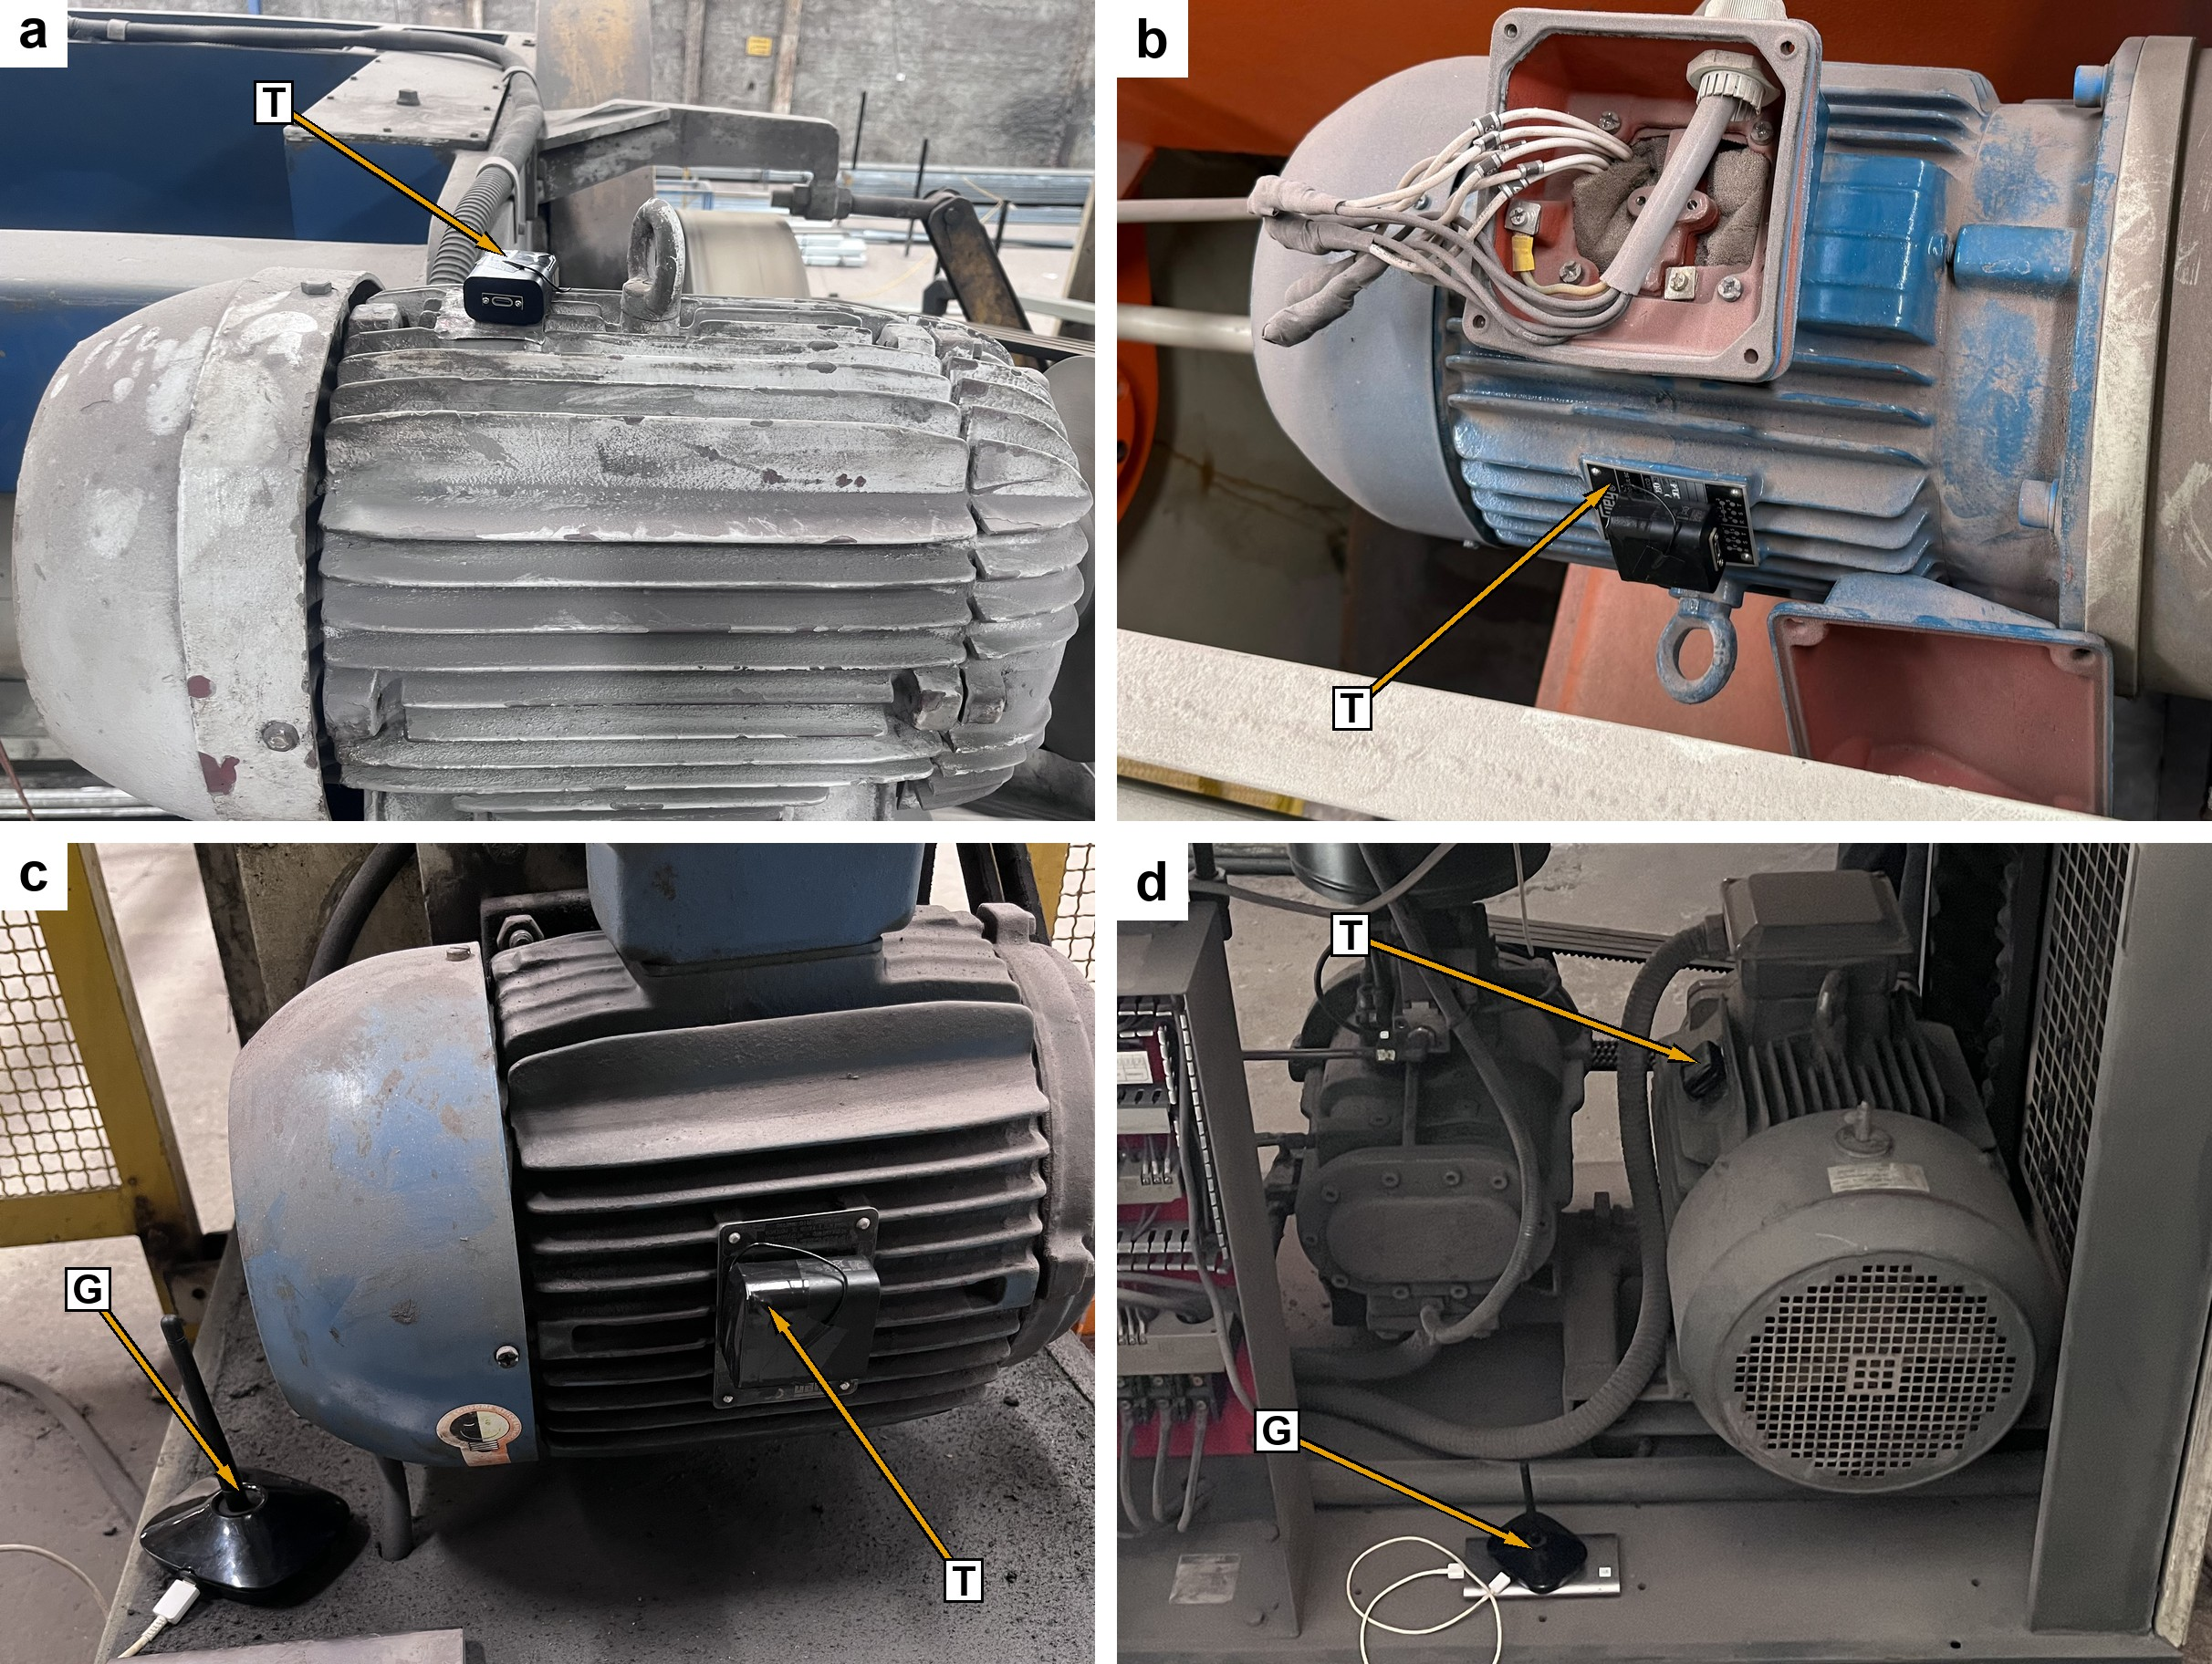
\includegraphics[width=\textwidth]{campo/fig16_montagem_campo.jpg}
\fonte{elaborado pelo próprio autor.}
\legenda{(a) dobradeira, às 12h45; (b) guilhotina, em horário não registrado; (c) calandra, às 13h17; (d) compressor, às 13h32. T indica o transmissor, e G, o \textit{gateway} na posição do momento da foto, apoiado sobre o carregador portátil que o alimentava.}
\end{figure}

Entre as duas rodadas, durante o almoço, o transmissor ficou ligado sobre uma mesa. Nesse período, a gravidade medida ficou constante, com o eixo Z na vertical, e o giroscópio não indicou movimento acima do próprio ruído. Por isso, as janelas adquiridas das \campoRepousoInicio\ às \campoRepousoFim\ foram usadas para estimar o ruído do sensor em repouso.

\section{Sistema de aquisição}\label{sec:sistema}

A coleta usou o sistema descrito na seção~\ref{cap:sistema}, com um transmissor e um \textit{gateway}. O transmissor usa um microcontrolador ESP32-C3, ligado a um módulo MPU-6050, com acelerômetro e giroscópio, por I2C e a um rádio Ra-02 (circuito SX1278) por SPI. O Ra-02 opera de \SIrange{410}{525}{\mega\hertz} \cite{aithinker2017ra02}. O \textit{gateway} usa um ESP32-S3 com o mesmo rádio, e a API e o banco de dados rodaram num computador levado ao local, na mesma rede Wi-Fi do \textit{gateway}.

O transmissor e o \textit{gateway} foram montados em invólucros reaproveitados (Figura~\ref{fig:dispositivos}). No transmissor, a placa ESP32-C3 Super Mini, o rádio, o módulo MPU-6050 e um módulo de carga de bateria TP4056 estão empilhados em um bloco, com as partes sensíveis protegidas por fita isolante líquida e fita de poliimida (Kapton). O invólucro é a carcaça vazia de um carregador, e dentro dele ficam o bloco, espumas entre o bloco e o invólucro e uma bateria de polímero de lítio de \SI{3,7}{\volt} e \SI{700}{\milli\ampere\hour}. A antena do rádio do transmissor é o fio que acompanha o módulo, no comprimento original. O invólucro do \textit{gateway} é a base de um sensor Kinect da primeira versão. Dentro dela ficam a placa de desenvolvimento do ESP32-S3, com o módulo coberto por fita de poliimida, e o rádio, em uma placa adaptadora, com os fios entre as duas placas agrupados por espaguete termorretrátil. Os dois rádios operam em \SI{433}{\mega\hertz}, e o do \textit{gateway} usou uma antena do tipo bastão feita para \SI{2,4}{\giga\hertz} e \SI{5}{\giga\hertz}, ligada ao módulo por um cabo com conector IPEX.

\begin{figure}[!htb]
\centering
\caption{Transmissor e \textit{gateway} usados na coleta em campo}\label{fig:dispositivos}
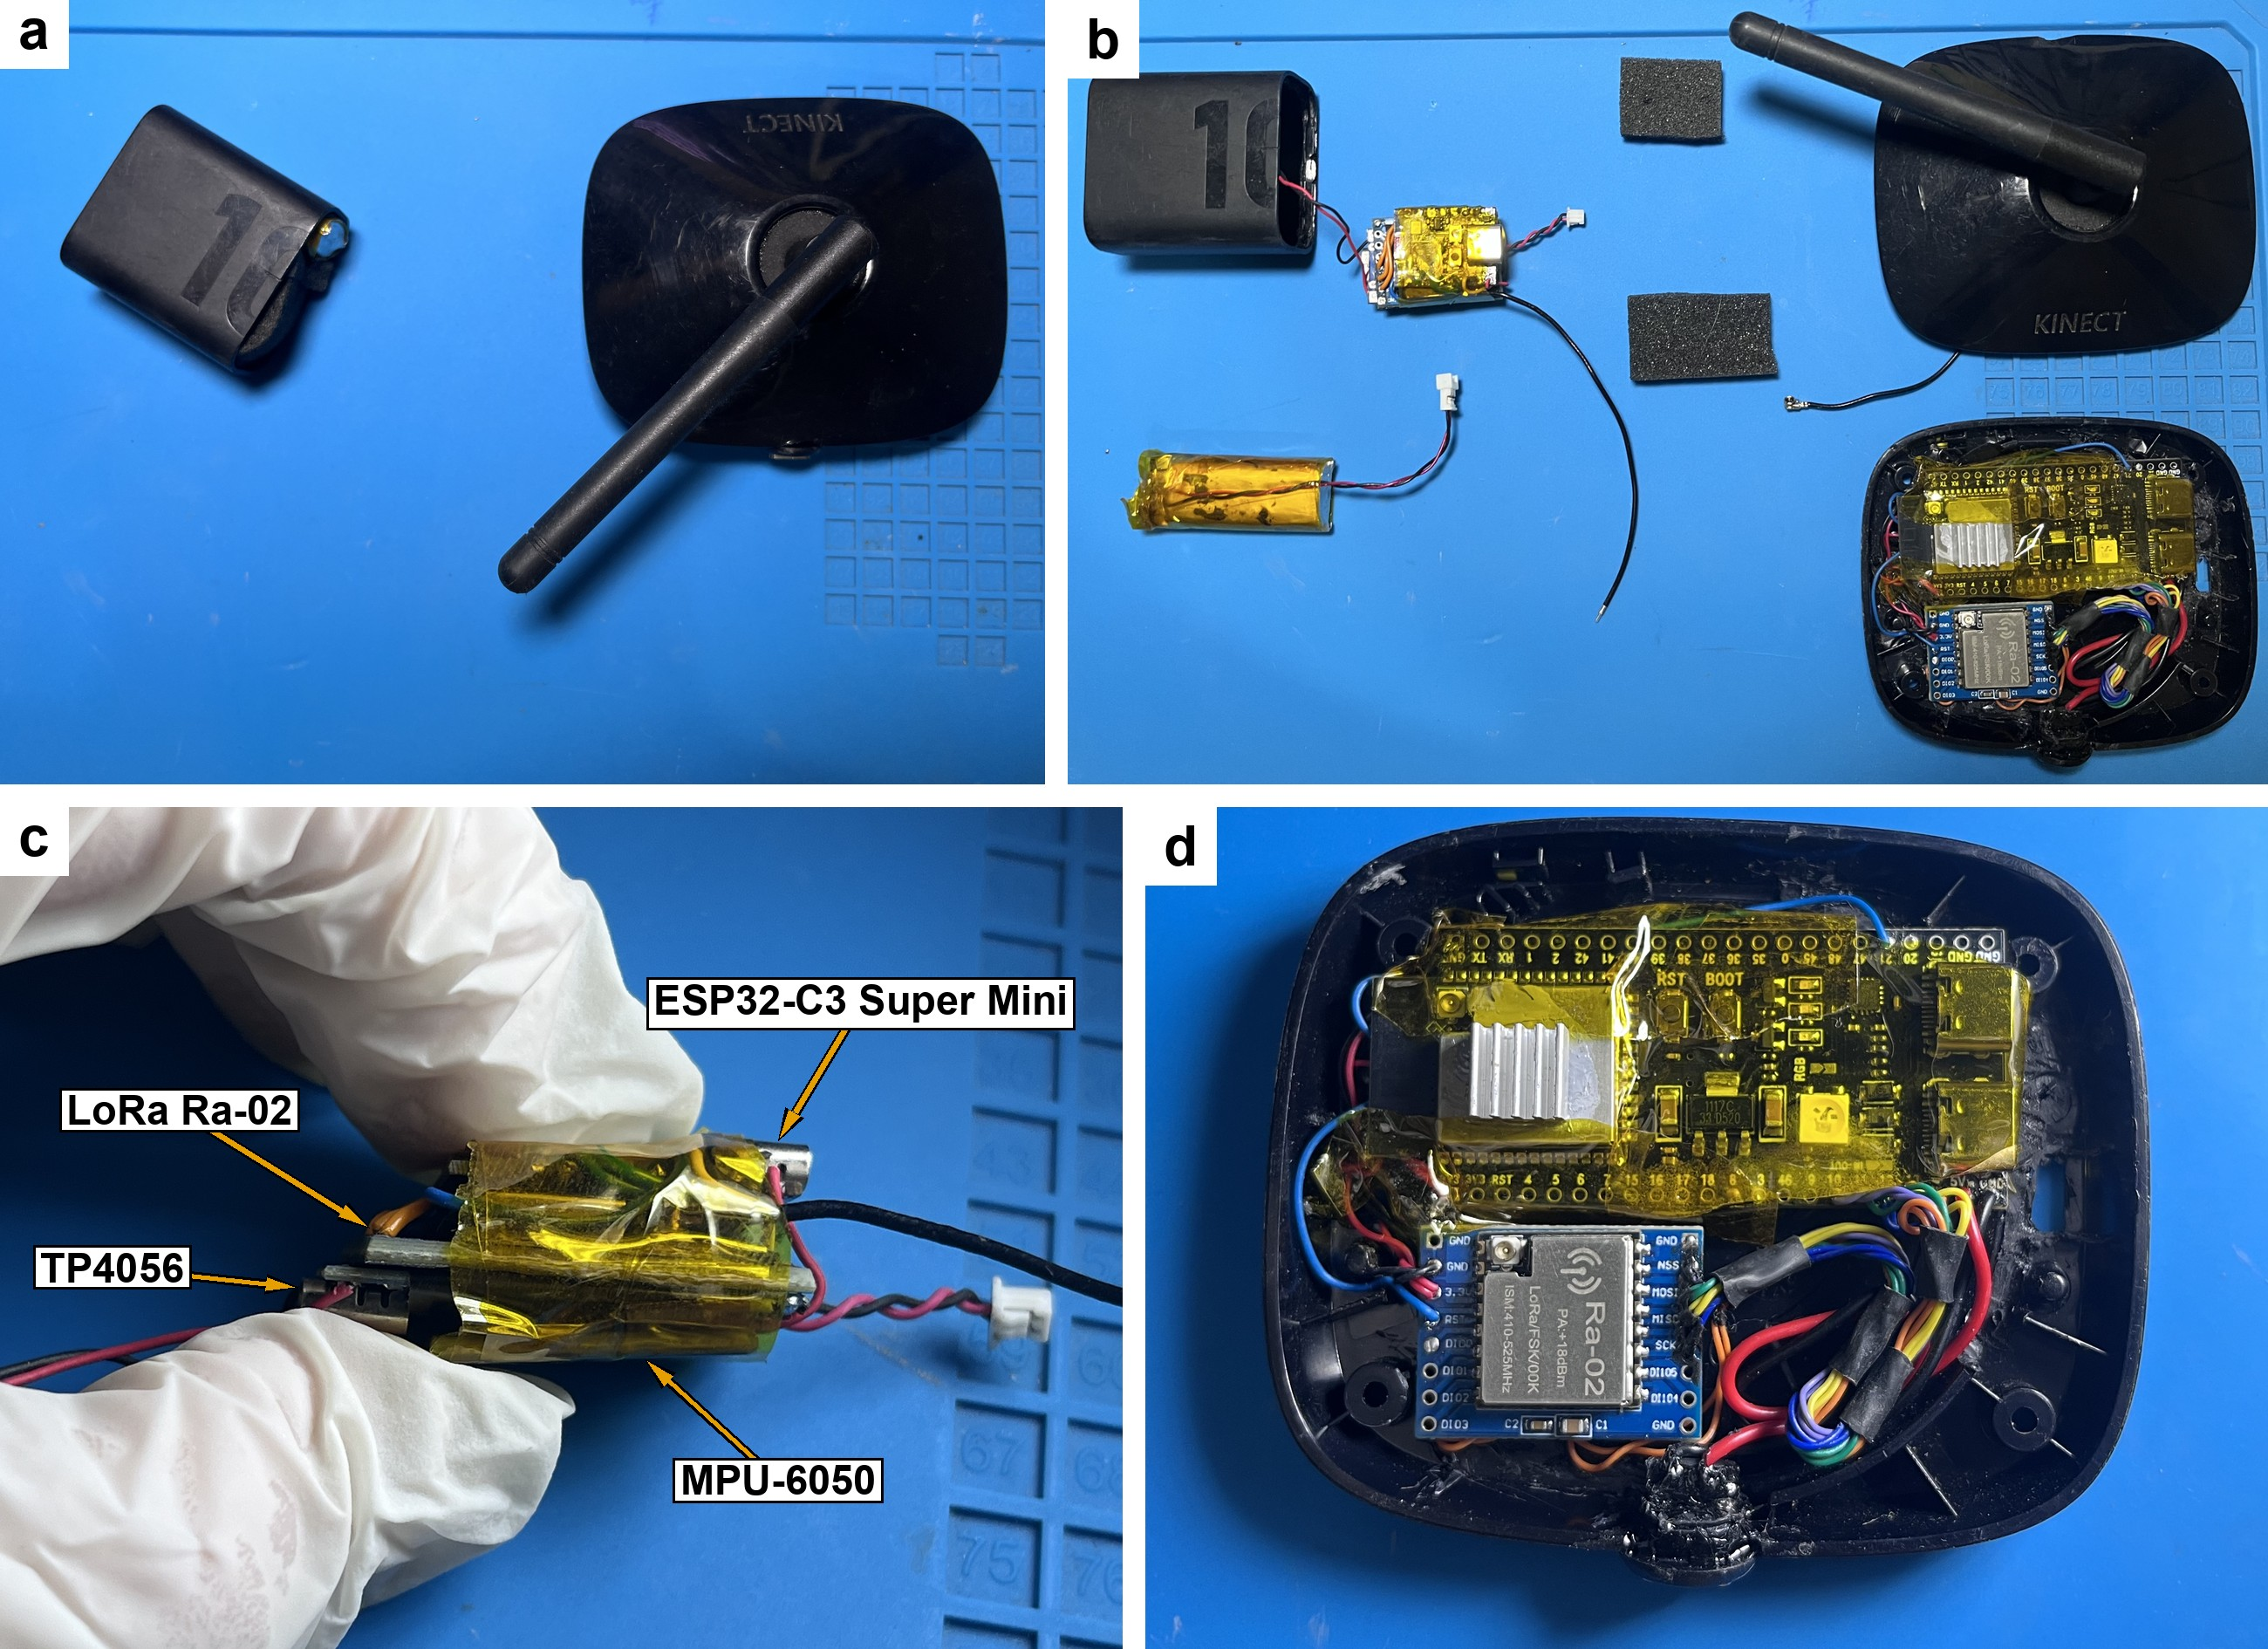
\includegraphics[width=\textwidth]{campo/fig20_dispositivos.jpg}
\fonte{elaborado pelo próprio autor.}
\legenda{(a) transmissor, à esquerda, e \textit{gateway}, à direita, fechados; (b) peças do transmissor, à esquerda e ao centro (invólucro, bloco eletrônico, bateria e espumas), e do \textit{gateway}, à direita (base e interior); (c) bloco eletrônico do transmissor, com os componentes indicados; (d) interior do \textit{gateway}, com a placa do ESP32-S3 coberta por fita de poliimida e o rádio na placa adaptadora. Fotos de 7 de novembro de 2026, cinco dias depois da coleta.}
\end{figure}

Os componentes eletrônicos dos dois dispositivos foram comprados no AliExpress. O preço pago não foi registrado, e a Tabela~\ref{tab:custo} dá o custo de uma compra nova, pela mediana dos preços anunciados para uma unidade em 9 de novembro de 2026, com os impostos. O pedido completo, de R\$~\num{140,83}, equivale a US\$~\num{25,60} pela taxa de câmbio de venda de 6 de novembro de 2026, de R\$~\num{5,5013} \cite{bcb2026ptax}. Desde 12 de maio de 2026, a compra de até US\$~\num{50} numa empresa certificada no Programa Remessa Conforme, como o AliExpress, tem imposto de importação zero \cite{receita2026manual}. Resta o ICMS, cuja carga nas remessas para o Piauí é de \SI{20}{\percent} \cite{piaui2025decreto}. Como o imposto é calculado por dentro, sobre o valor da compra somado ao próprio imposto, ele acrescenta \SI{25}{\percent} ao preço. A placa adaptadora do rádio do \textit{gateway} só é vendida em conjunto com o Ra-02, e o conjunto entrou na tabela no lugar do módulo avulso. Com o imposto, o transmissor custou R\$~\num{78,11} e o \textit{gateway}, R\$~\num{97,93}, sem a bateria, cujo preço não foi conferido.

\begin{table}[!htb]
\centering\small
\caption{Custo dos componentes do transmissor e do \textit{gateway} em 9 de novembro de 2026}\label{tab:custo}
\begin{tabular}{@{}llrrr@{}}
\toprule
Componente & Dispositivo & Anúncios & Preço (R\$) & Com ICMS (R\$) \\
\midrule
ESP32-C3 Super Mini & transmissor & \num{21} & \num{17,89} & \num{22,36} \\
Ra-02 (SX1278, \SI{433}{\mega\hertz}) & transmissor & \num{35} & \num{23,99} & \num{29,99} \\
Módulo MPU-6050 (GY-521) & transmissor & \num{39} & \num{13,69} & \num{17,11} \\
Módulo de carga TP4056 & transmissor & \num{13} & \num{6,92} & \num{8,65} \\
Bateria LiPo de \SI{3,7}{\volt} e \SI{700}{\milli\ampere\hour} & transmissor & 0 & \multicolumn{2}{c}{não cotada} \\
\addlinespace
\textit{Subtotal do transmissor} & & & \num{62,49} & \num{78,11} \\
\midrule
ESP32-S3 N16R8 (DevKitC-1) & \textit{gateway} & \num{19} & \num{31,29} & \num{39,11} \\
Ra-02 com placa adaptadora (conjunto) & \textit{gateway} & 1 & \num{27,99} & \num{34,99} \\
Antena de \num{2,4} e \SI{5}{\giga\hertz} com cabo IPEX & \textit{gateway} & \num{3} & \num{19,06} & \num{23,83} \\
\addlinespace
\textit{Subtotal do gateway} & & & \num{78,34} & \num{97,93} \\
\midrule
Total & & & \num{140,83} & \num{176,04} \\
\bottomrule
\end{tabular}
\fonte{elaborada pelo próprio autor, com preços do AliExpress e alíquotas de \citeonline{receita2026manual} e \citeonline{piaui2025decreto}.}
\nota{preço: mediana dos anúncios de uma unidade, de vendedores com envio do exterior, sem as ofertas de primeira compra; a coluna Anúncios dá quantos entraram na mediana. O frete foi considerado zero, porque a maioria dos anúncios o oferecia grátis. O conjunto do Ra-02 com placa adaptadora tem um só anúncio, de R\$~\num{27,99} na página do produto, com preço cheio de R\$~\num{56,00}. A consulta coincidiu com a campanha promocional de 11 de novembro. Com ICMS: carga de \SI{20}{\percent} calculada por dentro, igual a \SI{25}{\percent} do preço, e imposto de importação zero. Ficaram fora os invólucros reaproveitados, as fitas, as espumas e o computador da API.}
\end{table}

O sensor do módulo respondeu ao registrador de identificação (\texttt{WHO\_AM\_I}) com o valor \texttt{0x74}, diferente do \texttt{0x68} indicado no mapa de registradores do MPU-6050 \cite{invensense2012rm}, e a marcação do chip não foi conferida. O \textit{firmware} aceita os dois valores e, com \texttt{0x74}, usa o perfil MPU6515, em que o sensor foi configurado com faixa de $\pm\SI{4}{g}$ no acelerômetro, $\pm\SI{250}{\degree\per\second}$ no giroscópio e filtro passa-baixas digital interno de \SI{184}{\hertz} \cite{invensense2012rm}. A banda de \SI{184}{\hertz} é a nominal do mapa de registradores, e a resposta em frequência do sensor deste módulo não foi medida. O sensor amostra os seis canais a \SI{1}{\kilo\hertz} e guarda as amostras na FIFO, que o \textit{firmware} esvazia em lotes; assim, o espaçamento entre amostras é dado pelo relógio do sensor (seção~\ref{sec:sis-transmissor}). Cada janela tem \num{512} amostras por canal. O \textit{firmware} estima a taxa de amostragem de cada janela e, quando o desvio em relação a \SI{1}{\kilo\hertz} passa de \SI{2}{\percent}, marca a telemetria com código de diagnóstico e envia a janela com a taxa estimada.

Na coleta, o transmissor enviou em cada ciclo a telemetria e a janela de sinal bruto, no perfil padrão da rajada, com fator de espalhamento 7 e banda de \SI{250}{\kilo\hertz} (seção~\ref{sec:sis-protocolo}). A potência de transmissão foi de \campoPotenciaTx~dBm, abaixo do máximo do módulo em \SI{433}{\mega\hertz}, de \SI{18 \pm 1}{dBm} \cite{aithinker2017ra02}, e foi ajustada pelo rádio, como as demais mudanças de configuração (seção~\ref{sec:sis-configuracao}).

\section{Conjuntos de dados exportados}\label{sec:dados}

Os dados foram exportados do banco da API em modo somente leitura, e o resumo SHA-256 de cada janela foi conferido na exportação. O conjunto principal tem as \campoJanelas\ janelas e as \campoLeituras\ telemetrias dos trechos da Tabela~\ref{tab:ensaios}. Dois conjuntos complementares descrevem a medição em repouso e o enlace de rádio. O primeiro tem as \campoJanelasRepouso\ janelas com o transmissor sobre a mesa, e o segundo, \campoRajadas\ rajadas do histórico de eventos do \textit{gateway}, das \campoRajadasInicio\ às \campoRajadasFim, com o número de fragmentos recebidos e a duração de cada uma. Esse histórico guarda só os eventos mais recentes, e as rajadas anteriores às \campoRajadasInicio, inclusive as da dobradeira e da primeira rodada da guilhotina, não estão nele. O resumo SHA-256 do conjunto principal foi gravado no registro das hipóteses antes do cálculo (seção~\ref{sec:hipoteses}) e conferido no início de cada análise.

\section{Descritores}\label{sec:descritores}

As amostras do acelerômetro foram convertidas para $g$ pela faixa configurada, e a média de cada eixo foi removida em cada janela. A velocidade foi obtida por integração no domínio da frequência \cite{brandt2014}, sem janela de ponderação, com cada coeficiente $A_k$ da transformada discreta de Fourier da aceleração, na frequência $f_k$, dividido por $\mathrm{j}2\pi f_k$ e com os coeficientes fora da faixa de \SIrange{10}{184}{\hertz} anulados. O limite superior é o do filtro do sensor. A velocidade eficaz nessa faixa não é a de banda larga da norma, que vai até \SI{1000}{\hertz}, e não serve para classificar as máquinas nas zonas de severidade.

A rotação $f_r$ de cada janela foi estimada pelo maior pico do espectro da aceleração somado nos três eixos, com janela de Hann e preenchimento com zeros até \num{16} vezes o tamanho da janela, na faixa de $\pm\SI{2,5}{\hertz}$ em torno de um valor de busca fixado para cada máquina. Os valores de busca vieram das análises exploratórias (seção~\ref{sec:preliminares}): \campoBuscaDobradeiraUm~Hz na dobradeira e na calandra, \campoBuscaGuilhotinaUm~Hz na guilhotina e \campoBuscaCompressorUm~Hz no compressor. Nas três primeiras, a faixa de busca contém as rotações nominais das placas da guilhotina e da calandra. O compressor não tem dados de placa, e o valor de busca supõe que o pico perto de \SI{60}{\hertz} seja a rotação de um motor de dois polos. Com janelas de \SI{0,512}{\second}, a resolução do espectro é de \SI{1,95}{\hertz}, e o preenchimento com zeros não separa essa linha da frequência da rede elétrica, de \SI{60}{\hertz}.

Como a orientação do sensor mudou entre ensaios, os seis descritores de cada janela não dependem do sentido nem da ordem dos eixos:
\begin{itemize}
  \item $d_1$: velocidade eficaz de \SIrange{10}{184}{\hertz}, a maior entre os três eixos, em \si{\milli\meter\per\second};
  \item $d_2$: valor eficaz total da aceleração, raiz da soma dos quadrados dos três eixos, em $g$;
  \item $d_3$: maior curtose em excesso entre os três eixos;
  \item $d_4$: maior fator de crista entre os três eixos;
  \item $d_5$: amplitude eficaz da componente na rotação (ordem 1x) em velocidade, raiz da soma dos quadrados dos três eixos, em \si{\milli\meter\per\second};
  \item $d_6$: o mesmo para o dobro da rotação (ordem 2x).
\end{itemize}
As amplitudes $d_5$ e $d_6$ foram lidas no espectro com janela de Hann, corrigido para a perda de amplitude da janela. Nos detectores, $d_1$, $d_2$, $d_5$ e $d_6$ entram em logaritmo decimal.

\section{Detectores e limiar}\label{sec:detectores}

A linha de base de cada máquina é o conjunto de janelas de treino da operação normal, e um detector compara cada janela nova com ela. O detector principal é o Isolation Forest \cite{liu2008}, na implementação do scikit-learn \cite{scikitlearn2026}, com \num{100} árvores, subamostras do tamanho do treino até o máximo de \num{256} janelas e a semente do gerador de números aleatórios fixada em 0. O escore de cada janela é o oposto do valor devolvido por \texttt{score\_samples}, de modo que um escore maior indica janela mais afastada da linha de base. O detector secundário, usado só como descrição, é a regra por mediana e desvio absoluto mediano (MAD) \cite{leys2013}: o escore de uma janela é o maior valor, entre os seis descritores, de $|x - \tilde{x}|/(1{,}4826\,\mathrm{MAD})$, com a mediana $\tilde{x}$ e o MAD calculados no treino.

O limiar foi fixado para uma taxa de falso alarme de \SI{5}{\percent} na própria linha de base. As janelas de treino foram divididas em cinco blocos de janelas consecutivas, e cada bloco recebeu o escore de um modelo ajustado nos outros quatro. O limiar é o quantil de \SI{95}{\percent} desses escores, e o modelo usado na avaliação foi ajustado em todo o treino. Uma janela é marcada quando o escore passa do limiar.

\section{Assinaturas de desbalanceamento injetadas}\label{sec:injecao}

Como nenhuma máquina tinha falha conhecida, a fração de falhas detectadas não pode ser medida nesses dados. Para estimá-la em função da severidade, uma assinatura de desbalanceamento foi somada a janelas reais de operação normal que não participaram do treino. O desbalanceamento produz uma força que gira com o eixo, na frequência de rotação \cite{randall2011livro}, e por isso a assinatura foi somada aos dois eixos radiais do sensor, em quadratura:
\begin{equation}
a_{r1}(t) \leftarrow a_{r1}(t) + A_a \sin(2\pi f_r t + \varphi), \qquad a_{r2}(t) \leftarrow a_{r2}(t) + A_a \cos(2\pi f_r t + \varphi),
\label{eq:injecao}
\end{equation}
em que $f_r$ é a rotação medida na própria janela, $\varphi$ é uma fase sorteada por janela e $A_a = \sqrt{2}\,A_v\,2\pi f_r$ é a amplitude de aceleração que corresponde à velocidade eficaz $A_v$ acrescentada em cada eixo. $A_v$ variou de 0 a \SI{2,8}{\milli\meter\per\second}, em passos de \SI{0,05}{\milli\meter\per\second}. Na calandra e na guilhotina, o treino foi a primeira rodada, e o teste, a segunda. Na dobradeira e no compressor, que têm uma rodada, o treino foi a primeira metade das janelas, em ordem de tempo, e o teste, a segunda.

Para cada amplitude, a fração marcada é a fração das janelas de teste com escore do detector principal acima do limiar do treino. A amplitude com \SI{50}{\percent} das janelas marcadas, $A_{50}$, foi obtida por interpolação linear entre os pontos da grade. Uma assinatura do dobro da rotação, somada ao eixo axial, foi calculada apenas como descrição. A assinatura somada não reproduz a modulação, a variação de fase ao longo do tempo nem o caminho de transmissão de uma falha real, e uma falha real pode ser mais fácil ou mais difícil de detectar que a assinatura.

\section{Desbalanceamento real em base pública}\label{sec:base-publica}

Como a coleta não teve máquina com falha, o detector também foi avaliado numa base pública com desbalanceamento real, medida numa bancada de laboratório da Fraunhofer-Gesellschaft (\citeauthoronline{mey2020}, \citeyear{mey2020}, \citeyear{mey2022dados}). A base, na versão 151.3, tem licença Creative Commons Atribuição 4.0, que exige a citação dos autores, do título e do identificador digital de objeto (DOI) e a indicação das modificações. Neste trabalho, as modificações são o uso exclusivo das medições 0D e 0E a 4E, o recorte por tensão constante e por rotação, a divisão em janelas e o corte em \SI{184}{\hertz}, descritos a seguir. Os dados modificados não foram redistribuídos. Como o repositório original estava fora do ar, as medições foram obtidas da cópia do Internet Archive de 14 de dezembro de 2022.

Na bancada, um motor de corrente contínua com comutação eletrônica (WEG~UE~511~T) gira um eixo de \SI{12}{\milli\meter}, apoiado num mancal de rolamento em bloco de aço galvanizado. O desbalanceamento é uma massa presa a um suporte de náilon impresso em 3D, montado logo atrás do bloco do mancal, em cinco níveis: 0, com o suporte sem massa, e 1 a 4, com \SIlist{45,9;60,7;75,5;152,1}{\milli\meter\gram}. Três acelerômetros uniaxiais PCB M607A11, no bloco do mancal e na fixação do motor, foram amostrados a \SI{4096}{\hertz}, e a base não informa a posição de cada canal nem a unidade da vibração. A rotação muda em degraus de tensão de \SI{20}{\second}, percorridos duas vezes. Nos arquivos de desenvolvimento, 0D a 4D, a tensão vai de \SIrange{2,0}{10,05}{\volt} em passos de \SI{0,05}{\volt}, e nos de avaliação, 0E a 4E, de \SIrange{4,0}{8,1}{\volt} em passos de \SI{0,1}{\volt}. Entre as medições D e E, o suporte do desbalanceamento foi desmontado e remontado.

Os primeiros \num{50000} valores de cada arquivo foram descartados, como no artigo da base \cite{mey2020}. Depois do descarte, o número de amostras de 0E e de 4E coincidiu com o informado nos cadernos dos autores da base, conferência prevista no registro de H4 (Apêndice~\ref{ap:registro}). O sinal foi dividido em janelas consecutivas, sem sobreposição, de \num{2048} amostras, que duram \SI{0,5}{\second} e têm resolução de \SI{2,0}{\hertz}, perto das janelas do transmissor, de \SI{0,512}{\second} e \SI{1,95}{\hertz}. Entraram as janelas com tensão constante e rotação média de \SIrange{1750}{1850}{r/min}, faixa que contém a rotação estimada na dobradeira, na guilhotina e na calandra, de \rotacaoRpmMin\ a \rotacaoRpmMax~r/min. As duas primeiras janelas de cada degrau, em que a rotação ainda muda, foram descartadas. Os três canais de vibração fazem o papel dos três eixos do sensor, com a média removida em cada janela. Para reproduzir a banda do transmissor, os coeficientes acima de \SI{184}{\hertz} foram anulados antes do cálculo de $d_2$, $d_3$ e $d_4$, e a velocidade de $d_1$ vai de \SIrange{10}{184}{\hertz}, como na seção~\ref{sec:descritores}. A rotação $f_r$ de cada janela é o pico do espectro da mesma seção, com valor de busca igual à média da rotação medida pela bancada na janela. Como a unidade da vibração não é informada, $d_1$, $d_2$, $d_5$ e $d_6$ ficam na unidade dos canais. O detector usa esses descritores em logaritmo, e um fator de escala comum ao treino e ao teste não muda o resultado.

O detector principal e o limiar são os da seção~\ref{sec:detectores}, com treino em todas as janelas do arquivo 0D que passaram pelo pré-processamento. O falso alarme é a fração das janelas de 0E marcadas, e a fração marcada em cada nível de desbalanceamento é a das janelas de 1E a 4E, com intervalos de confiança como na seção~\ref{sec:analise}. No download, o tamanho e o CRC-32 de cada arquivo foram conferidos com o índice do arquivo compactado, e o SHA-256 de cada um foi gravado antes do cálculo de qualquer descritor.

A bancada tem motor pequeno, eixo de \SI{12}{\milli\meter} e nenhuma carga, e os três sensores são uniaxiais e ficam em dois pontos, enquanto o transmissor usa um sensor triaxial num ponto. Nenhum ruído foi acrescentado ao sinal da base, e o sensor do transmissor não foi modelado. Por isso, H4 avalia o método de detecção diante de uma falha real, e o desempenho do dispositivo em campo continua avaliado só por H1 a H3.

\section{Hipóteses e critérios}\label{sec:hipoteses}

A hipótese central é que, com uma linha de base construída só com operação normal, a cadeia de aquisição de baixo custo da seção~\ref{sec:sistema}, do sensor à API, detecta mudanças de vibração do tamanho que a norma considera significativas, com falso alarme limitado entre rodadas da mesma máquina. Ela se desdobra em três hipóteses derivadas, H1 a H3 (Quadro~\ref{tab:hipoteses}). Uma quarta hipótese, H4, avalia o detector diante do desbalanceamento real da base pública (seção~\ref{sec:base-publica}). H1 a H3 e os critérios de decisão foram registrados em 6 de novembro de 2026, antes de qualquer cálculo que as avaliasse, e não mudaram depois dos resultados. Em 7 de novembro, uma emenda acrescentou H4 e duas análises posteriores aos resultados de H2 e H3, AP1 e AP2 (seção~\ref{sec:res-posteriores}), antes do cálculo delas. Outra emenda, também anterior ao cálculo de H4, trocou a versão da base pública, porque a versão 151.2 ficou indisponível. Em 8 de novembro, depois de todos esses resultados, uma terceira emenda acrescentou quatro análises posteriores, AP3 a AP6, sem hipótese nova e sem mudança de critério (seção~\ref{sec:res-posteriores}). O Apêndice~\ref{ap:registro} descreve cada registro e o que já se conhecia antes dele.

\begin{quadro}[!htb]
\centering\small
\caption{Hipóteses e critérios de corroboração e de refutação}\label{tab:hipoteses}
\begin{tabular}{@{}>{\raggedright\arraybackslash}p{36mm}>{\raggedright\arraybackslash}p{62mm}>{\raggedright\arraybackslash}p{46mm}@{}}
\toprule
Hipótese & Critério de corroboração & Critério de refutação \\
\midrule
H1. Falso alarme entre rodadas & Na calandra e na guilhotina, com treino na primeira rodada, o detector principal marca até \SI{10}{\percent} das janelas da segunda rodada, com limite superior do intervalo de até \SI{20}{\percent} & Fração marcada acima de \SI{20}{\percent} em ao menos uma das máquinas \\
\addlinespace
H2. Menor mudança detectável & Em todos os ensaios com ao menos \num{25} janelas, a menor mudança detectável em $d_1$ fica abaixo de \SI{0,7}{\milli\meter\per\second} & Menor mudança detectável de \SI{0,7}{\milli\meter\per\second} ou mais em ao menos um desses ensaios \\
\addlinespace
H3. Detecção da assinatura injetada & Nas quatro máquinas, $A_{50}$ fica abaixo de \SI{0,7}{\milli\meter\per\second}, e a correlação de Spearman entre a amplitude e a fração marcada é de \num{0,9} ou mais & $A_{50}$ de \SI{0,7}{\milli\meter\per\second} ou mais, ou não atingido até \SI{2,8}{\milli\meter\per\second}, ou correlação abaixo de \num{0,9}, em ao menos uma máquina \\
\addlinespace
H4. Desbalanceamento real em base pública & Com treino em 0D, o detector principal marca até \SI{10}{\percent} das janelas de 0E, com limite superior do intervalo de até \SI{20}{\percent}, e \SI{50}{\percent} ou mais das janelas em cada nível, de 1E a 4E & Fração marcada acima de \SI{20}{\percent} em 0E, ou abaixo de \SI{50}{\percent} em ao menos um nível \\
\bottomrule
\end{tabular}
\fonte{elaborado pelo próprio autor.}
\nota{em H1 e em H4, os resultados entre os dois critérios deixam a hipótese indeterminada. Em H2, a regra de alarme é $d_1$ acima do quantil de \SI{95}{\percent} de $d_1$ no próprio ensaio, e a menor mudança detectável é a diferença entre esse quantil e a mediana: o aumento da mediana que leva metade das janelas acima do limiar, com a dispersão mantida.}
\end{quadro}

A ISO 20816-3 avalia a vibração pelo valor da vibração de banda larga e pela mudança desse valor \cite{iso208163_2022}. Na série ISO 10816, que a ISO 20816-3 substituiu, uma variação de \SI{25}{\percent} do limite superior da zona B, para mais ou para menos, é considerada significativa e pede investigação da causa \cite{schwirzer2002}. Neste trabalho, o tamanho de referência é \SI{0,7}{\milli\meter\per\second}, \SI{25}{\percent} do limite B/C de \SI{2,8}{\milli\meter\per\second} do grupo 2 em fundação rígida, o menor limite B/C da norma. Pela edição de 2022 da norma, a guilhotina e a calandra, com \SI{9,2}{\kilo\watt} e \SI{2,2}{\kilo\watt}, ficam abaixo da potência mínima, de \SI{15}{\kilo\watt}, e nelas o valor serve só de referência de tamanho. A edição de 2026 não fixa potência mínima no escopo, e os limites de zona dessa edição não foram consultados (seção~\ref{sec:fund-norma}). O compressor, com \SI{22}{\kilo\watt}, está no grupo 2, de \SIrange{15}{300}{\kilo\watt}.

A hipótese central é corroborada quando H1, H2 e H3 o são. H4, avaliada na base pública, não entra nessa decisão.

\subsection{Análises exploratórias anteriores ao registro}\label{sec:preliminares}

Os mesmos dados foram examinados em 2 e 5 de novembro, antes do registro. Nessas análises exploratórias, com outro conjunto de descritores, o Isolation Forest e a regra por mediana e MAD foram treinados em uma rodada e aplicados à outra e marcaram, respectivamente, de \registroExplIfMin~\% a \registroExplIfMax~\% e de \registroExplMadMin~\% a \registroExplMadMax~\% das janelas. A velocidade eficaz da calandra e da guilhotina também foi comparada entre as rodadas, e a rotação e as ordens de cada máquina foram estimadas. Os limites de \SI{10}{\percent} e de \SI{20}{\percent} de H1 foram fixados depois dessas frações, e por isso a avaliação de H1 não é independente das análises exploratórias. Essas análises originaram as hipóteses e não as corroboram. A avaliação de H1 a H3 usou somente os dados de 2 de novembro, e não houve nova coleta.

\subsection{Procedimentos de validade}\label{sec:validade-proc}

O delineamento adotou procedimentos para cada um dos quatro aspectos de validade descritos por \citeonline[p.~153--154]{runeson2009}, e as ameaças que permaneceram são avaliadas na seção~\ref{sec:limitacoes}. Para a validade de construto, os descritores, os detectores e os critérios foram definidos antes do cálculo, a velocidade foi comparada com o critério da norma com a diferença de banda declarada, e a injeção da assinatura foi conferida numa janela sintética de fase conhecida (seção~\ref{sec:res-ap1}). Para a validade interna, os critérios foram registrados antes do cálculo, e a avaliação incluiu controles descritivos: o sentido inverso de H1, a regra por mediana e MAD, o motor desligado e o sensor em repouso. Para a validade externa, o detector foi aplicado também a uma base pública de laboratório com desbalanceamento real (seção~\ref{sec:base-publica}). Para a confiabilidade, os dados foram conferidos pelo resumo SHA-256 (seção~\ref{sec:dados}), as sementes do gerador de números aleatórios e as versões das bibliotecas foram fixadas, e os números do texto foram gravados pelas próprias análises.

\section{Análise estatística}\label{sec:analise}

As frações de janelas marcadas têm intervalo de confiança de \SI{95}{\percent} por reamostragem em blocos de cinco janelas consecutivas, com \num{2000} réplicas e percentis, porque janelas próximas no tempo não são independentes. Não houve correção de multiplicidade. A integridade dos dados foi descrita pelas lacunas na sequência das telemetrias, pela taxa de amostragem estimada pelo transmissor e pela conferência do SHA-256. Os cálculos foram feitos em Python \ambPython, com NumPy \ambNumpy, SciPy \ambScipy\ e scikit-learn \ambSklearn, e a avaliação de H4, também com pandas \ambPandas. A documentação do Isolation Forest citada neste trabalho \cite{scikitlearn2026} é a da versão 1.9.1, consultada em 29 de outubro de 2026. Os dados da coleta e o código do sistema e das análises estão nos repositórios do projeto.\plano{Endereço público e licença dos repositórios e dos dados: a definir pelo autor.}
